\subsection{Modeling Approach for Partial Models}

The full model is assembled from several partial models, which cover the most 
significant, i.e. time-demanding, regions of the ESPRESO solver. The partials models take
number of nodes \verb!nnodes!, number of processes per node \verb!nprocs!,
number of domains per node \verb!ndoms! and number of DOF per MPI process \verb!nDOF!
as inputs.

The partial models were created by generalized linear regression with natural logarithm as a link function to enforce positive values of the output variable (i.e. time). This was performed using R-language \cite{rDocs}
%, which is very briefly described in Appendix \ref{sec:r}.

In the rest of this section the modeling approach is explained on partial model describing the action of the stiffness matrix $K$ in HTFETI. The application of the HTFETI $\tilde{F}$-operator (which is not assembled explicitly in ESPRESO) is show in Eq. \eqref{eq:htfetiDualProblem}. 

The modeling itself is an iterative process. The first version of the model is shown in the Eq. \eqref{eq:actionKHTFETIFull}, containing 
polynomial of every predictor variable and all their interactions, so we do not omit anything. The variable $nprocs$ is described as a fraction $\frac{1}{nprocs}$, because data which depends on it lies on a hyperbola, which is caused by a significant NUMA effect (as described in \cite{molka2015cache}).


\begin{equation}
\label{eq:actionKHTFETIFull}
\begin{aligned}
t_{K|act|HT} \sim\; &\mathrm{(poly(I(1/nprocs), 2) + poly(ndoms, 2)}\\
&+ \mathrm{poly(nDOF, 2))\,\widehat{}\,3}
\end{aligned}
\end{equation}
The summary of the model (see Tab. \ref{tab:actionKHTFETI}) shows, that only some of the main effects  significantly contribute to the model. The proposed model fits much better then the null model, as can be seen from listed deviances. 
Also we can see, that Fisher scoring algorithm (described in \cite{fischerScoringAlg}), 
found some optima, because there is the finite number of its iterations.


\begin{table}[!hptb]
\centering
\scriptsize
%\resizebox{\textwidth}{!}{
\begin{tabular}{llllll}
 & \textbf{t value} & \textbf{Pr(\textgreater|t|)} & \textbf{} \\
\textbf{(Intercept)} & -85.758 & \textless 2e-16 & *** \\
\textbf{poly(I(1/nprocs), 2)1} & 1.244 & 0.21546 &  \\
\textbf{poly(I(1/nprocs), 2)2} & -0.188 & 0.85098 &  \\
\textbf{poly(ndoms, 2)1} & 21.908 & \textless 2e-16 & *** \\
\textbf{poly(ndoms, 2)2} & -3.227 & 0.00155 & ** \\
\textbf{poly(nDOF, 2)1} & 47.715 & \textless 2e-16 & *** \\
\textbf{poly(nDOF, 2)2} & -19.592 & \textless 2e-16 & *** \\
\textbf{poly(I(1/nprocs), 2)1:poly(ndoms, 2)1} & 0.036 & 0.97125 &  \\
\textbf{\vdots} & \vdots & \vdots &  \\
\textbf{poly(I(1/nprocs), 2)1:poly(ndoms, 2)1:poly(nDOF, 2)1} & -0.045 & 0.96445 &  \\
\textbf{\vdots} & \vdots & \vdots &  \\
\hhline{====}
\textbf{Null deviance} & \multicolumn{1}{r}{9.766522 (167DOF)} &  &  \\
\textbf{Residual deviance} & \multicolumn{1}{r}{0.030749 (141DOF)} &  &  \\
\textbf{AIC} & \multicolumn{1}{r}{-913.02} &  &  \\
\textbf{Fisher Scoring it.} & \multicolumn{1}{r}{6} &  & 
\end{tabular}
%}
\caption{Action of $K$ - HTFETI (1st model)}
\label{tab:actionKHTFETI}
\vspace{1.5em}
\scriptsize
%\resizebox{\textwidth}{!}{
\begin{tabular}{llllll}
 & \textbf{Estimate} & \textbf{Std. Error} & \textbf{t value} & \textbf{Pr(\textgreater|t|)} &  \\
\textbf{(Intercept)} & -2.63321 & 0.01217 & -216.33 & \textless 2e-16 & *** \\
\textbf{I(1/nprocs)} & 0.05772 & 0.01081 & 5.34 & 3.14e-07 & *** \\
\textbf{poly(ndoms, 3)1} & 6.70538 & 0.02693 & 248.99 & \textless 2e-16 & *** \\
\textbf{poly(ndoms, 3)2} & -1.18015 & 0.03270 & -36.09 & \textless 2e-16 & *** \\
\textbf{poly(ndoms, 3)3} & 0.15667 & 0.03775 & 4.15 & 5.38e-05 & *** \\
\textbf{poly(nDOF, 3)1} & 16.45273 & 0.13900 & 118.37 & \textless 2e-16 & *** \\
\textbf{poly(nDOF, 3)2} & -4.97680 & 0.10190 & -48.84 & \textless 2e-16 & *** \\
\textbf{poly(nDOF, 3)3} & 1.30552 & 0.05489 & 23.79 & \textless 2e-16 & *** \\
\hhline{======}
\textbf{Null deviance} & \multicolumn{1}{r}{9.7665223  (167 DOF)} &  &  &  &  \\
\textbf{Residual deviance} & \multicolumn{1}{r}{0.0056578 (160 DOF)} &  &  &  &  \\
\textbf{AIC} & \multicolumn{1}{r}{-1235.4} &  &  &  &  \\
\textbf{Fisher Scoring it.} & \multicolumn{1}{r}{5} &  &  &  & 
\end{tabular}
%}
\caption{Action of $K$ - HTFETI (improved model)}
\label{tab:actionKHTFETIimp}
\vspace{1.5em}
\scriptsize
%\resizebox{\textwidth}{!}{
\begin{tabular}{llllll}
\multicolumn{1}{c}{} & \textbf{Estimate} & \textbf{Std. Error} & \textbf{t value} & \textbf{Pr(\textgreater|t|)} & \multicolumn{1}{c}{} \\
\textbf{(Intercept)} & -6.693e+00 & 1.168e-01 & -57.284 & \textless 2e-16 & *** \\
\textbf{I(1/nprocs)} & 5.772e-02 & 1.081e-02 & 5.340 & 3.14e-07 & *** \\
\textbf{poly(ndoms, 3, raw = T)1} & 6.047e-03 & 6.210e-04 & 9.738 & \textless 2e-16 & *** \\
\textbf{poly(ndoms, 3, raw = T)2} & -5.647e-06 & 1.046e-06 & -5.398 & 2.39e-07 & *** \\
\textbf{poly(ndoms, 3, raw = T)3} & 2.126e-09 & 5.123e-10 & 4.150 & 5.38e-05 & *** \\
\textbf{poly(nDOF, 3, raw = T)1} & 7.290e-04 & 1.524e-05 & 47.847 & \textless 2e-16 & *** \\
\textbf{poly(nDOF, 3, raw = T)2} & -5.256e-08 & 1.759e-09 & -29.874 & \textless 2e-16 & *** \\
\textbf{poly(nDOF, 3, raw = T)3} & 1.473e-12 & 6.193e-14 & 23.785 & \textless 2e-16 & *** \\ \hhline{======}
\textbf{Null deviance} & \multicolumn{1}{r}{9.7665223 (167 DOF)} &  &  &  &  \\
\textbf{Residual deviance} & \multicolumn{1}{r}{0.0056578 (160 DOF)} &  &  &  &  \\
\textbf{AIC} & \multicolumn{1}{r}{-1235.4} &  &  &  &  \\
\textbf{Fisher Scoring it.} & \multicolumn{1}{r}{5} &  &  &  & \\
\hhline{======}
\multicolumn{2}{c}{\textbf{Cross-validation}} &  &  &  &  \\
\textbf{mean(RMSE)} & \multicolumn{1}{r}{0.005745} &  &  &  &  \\
\textbf{sd(RMSE)} & \multicolumn{1}{r}{0.001180} &  &  &  &  \\
\textbf{mean(MAPE)} & \multicolumn{1}{r}{0.158468} &  &  &  &  \\
\textbf{sd(MAPE)} & \multicolumn{1}{r}{0.037536} &  &  &  &
\end{tabular}
%}
\caption{Action of $K$ - HTFETI (final model)}
\label{tab:actionKHTFETIFinal}
\end{table}


So, in the next step we will remove all the interactions and the quadratic term of the $nprocs$ 
polynomial, because, as we can see in the summary, it is marked as non-significant too. 
The linear term of this polynomial has also high p-value, but it is not convenient to remove all the main effects of some predictor variable just because of the Wald test. The reason is that after removing 
some terms the remaining ones can be already detected as significant ones. And even if the 
remaining main effects would not be detected as significant by the Wald test, the model has usually 
better predictive capability with the main effects included for all predictor variables.


The new model is described as
\begin{equation}
\label{eq:actionKHTFETIimp}
t_{K|act|HT} \sim\; \mathrm{I(1/nprocs) + poly(ndoms, 3) + poly(nDOF, 3)\,.}
\end{equation}
As we can see in the Tab. \ref{tab:actionKHTFETIimp}, all the terms in the model are now detected as significant by Wald test. Akaike information criterion (AIC) is much lower than previous -913.02, which denotes the significant
improvement of the model. Moreover the residual deviance is significantly lower than the null deviance, which means great improvement over the null model, i.e. the well-fitting model on the data-set.

% \begin{table}[H]
% \centering
% \resizebox{\textwidth}{!}{
% \begin{tabular}{llllll}
%  & \textbf{Estimate} & \textbf{Std. Error} & \textbf{t value} & \textbf{Pr(\textgreater|t|)} &  \\
% \textbf{(Intercept)} & -2.63321 & 0.01217 & -216.33 & \textless 2e-16 & *** \\
% \textbf{I(1/nprocs)} & 0.05772 & 0.01081 & 5.34 & 3.14e-07 & *** \\
% \textbf{poly(ndoms, 3)1} & 6.70538 & 0.02693 & 248.99 & \textless 2e-16 & *** \\
% \textbf{poly(ndoms, 3)2} & -1.18015 & 0.03270 & -36.09 & \textless 2e-16 & *** \\
% \textbf{poly(ndoms, 3)3} & 0.15667 & 0.03775 & 4.15 & 5.38e-05 & *** \\
% \textbf{poly(nDOF, 3)1} & 16.45273 & 0.13900 & 118.37 & \textless 2e-16 & *** \\
% \textbf{poly(nDOF, 3)2} & -4.97680 & 0.10190 & -48.84 & \textless 2e-16 & *** \\
% \textbf{poly(nDOF, 3)3} & 1.30552 & 0.05489 & 23.79 & \textless 2e-16 & *** \\
% \hhline{======}
% \textbf{Null deviance} & \multicolumn{1}{r}{9.7665223  (167 DOF)} &  &  &  &  \\
% \textbf{Residual deviance} & \multicolumn{1}{r}{0.0056578 (160 DOF)} &  &  &  &  \\
% \textbf{AIC} & \multicolumn{1}{r}{-1235.4} &  &  &  &  \\
% \textbf{Fisher Scoring it.} & \multicolumn{1}{r}{5} &  &  &  & 
% \end{tabular}
% }
% \caption{Action of $K$ - HTFETI (improved model)}
% \label{tab:actionKHTFETIimp}
% \end{table}

So, we can change the model to use ordinary polynomials as 

\begin{equation}
\label{eq:actionKHTFETIFfinal}
\begin{aligned}
t_{K|act|HT} \sim\; &\mathrm{I(1/nprocs) + poly(ndoms, 3, raw=T)}\\
&+ \mathrm{poly(nDOF, 3, raw=T)}
\end{aligned}
\end{equation}
and perform cross-validation to evaluate the predictive capability of the model. The estimated coefficients are listed in Tab. \ref{tab:actionKHTFETIFinal}.

% \begin{table}[H]
% \centering
% \resizebox{\textwidth}{!}{
% \begin{tabular}{llllll}
% \multicolumn{1}{c}{} & \textbf{Estimate} & \textbf{Std. Error} & \textbf{t value} & \textbf{Pr(\textgreater|t|)} & \multicolumn{1}{c}{} \\
% \textbf{(Intercept)} & -6.693e+00 & 1.168e-01 & -57.284 & \textless 2e-16 & *** \\
% \textbf{I(1/nprocs)} & 5.772e-02 & 1.081e-02 & 5.340 & 3.14e-07 & *** \\
% \textbf{poly(ndoms, 3, raw = T)1} & 6.047e-03 & 6.210e-04 & 9.738 & \textless 2e-16 & *** \\
% \textbf{poly(ndoms, 3, raw = T)2} & -5.647e-06 & 1.046e-06 & -5.398 & 2.39e-07 & *** \\
% \textbf{poly(ndoms, 3, raw = T)3} & 2.126e-09 & 5.123e-10 & 4.150 & 5.38e-05 & *** \\
% \textbf{poly(nDOF, 3, raw = T)1} & 7.290e-04 & 1.524e-05 & 47.847 & \textless 2e-16 & *** \\
% \textbf{poly(nDOF, 3, raw = T)2} & -5.256e-08 & 1.759e-09 & -29.874 & \textless 2e-16 & *** \\
% \textbf{poly(nDOF, 3, raw = T)3} & 1.473e-12 & 6.193e-14 & 23.785 & \textless 2e-16 & *** \\ \hhline{======}
% \textbf{Null deviance} & \multicolumn{1}{r}{9.7665223 (167 DOF)} &  &  &  &  \\
% \textbf{Residual deviance} & \multicolumn{1}{r}{0.0056578 (160 DOF)} &  &  &  &  \\
% \textbf{AIC} & \multicolumn{1}{r}{-1235.4} &  &  &  &  \\
% \textbf{Fisher Scoring it.} & \multicolumn{1}{r}{5} &  &  &  & \\
% \hhline{======}
% \multicolumn{2}{c}{\textbf{Cross-validation}} &  &  &  &  \\
% \textbf{mean(RMSE)} & \multicolumn{1}{r}{0.005745} &  &  &  &  \\
% \textbf{sd(RMSE)} & \multicolumn{1}{r}{0.001180} &  &  &  &  \\
% \textbf{mean(MAPE)} & \multicolumn{1}{r}{0.158468} &  &  &  &  \\
% \textbf{sd(MAPE)} & \multicolumn{1}{r}{0.037536} &  &  &  &
% \end{tabular}
% }
% \caption{Action of $K$ - HTFETI (final model)}
% \label{tab:actionKHTFETIFinal}
% \end{table}


As we can see, the coefficients differ dramatically from the previous 
ones, but all the terms significantly contribute to the model. Predicted
values did not change, as we can see from the null deviance, residual
deviance and AIC being the same. We can see the visualized fit on the all 
data-set used for training in Fig. \ref{fig:actionK-HTFETI}. There were performed 15 iterations of repeated random sub-sampling cross-validation. The results are 
listed in the Tab. 
\ref{tab:actionKHTFETIFinal}.
% and visualized in Fig. \ref{fig:actionK-HTFETI-crossVal}.
As we can see, expected values of RMSE and MAPE are pretty low and their 
standard deviations are low too. Therefore the predictive capability of this
model is good and it does not tend to worsen significantly for some 
training sets.


\begin{figure}[htb]
\centering
%\adjustbox{max width=\linewidth}{
%\begin{minipage}{0.6\linewidth}
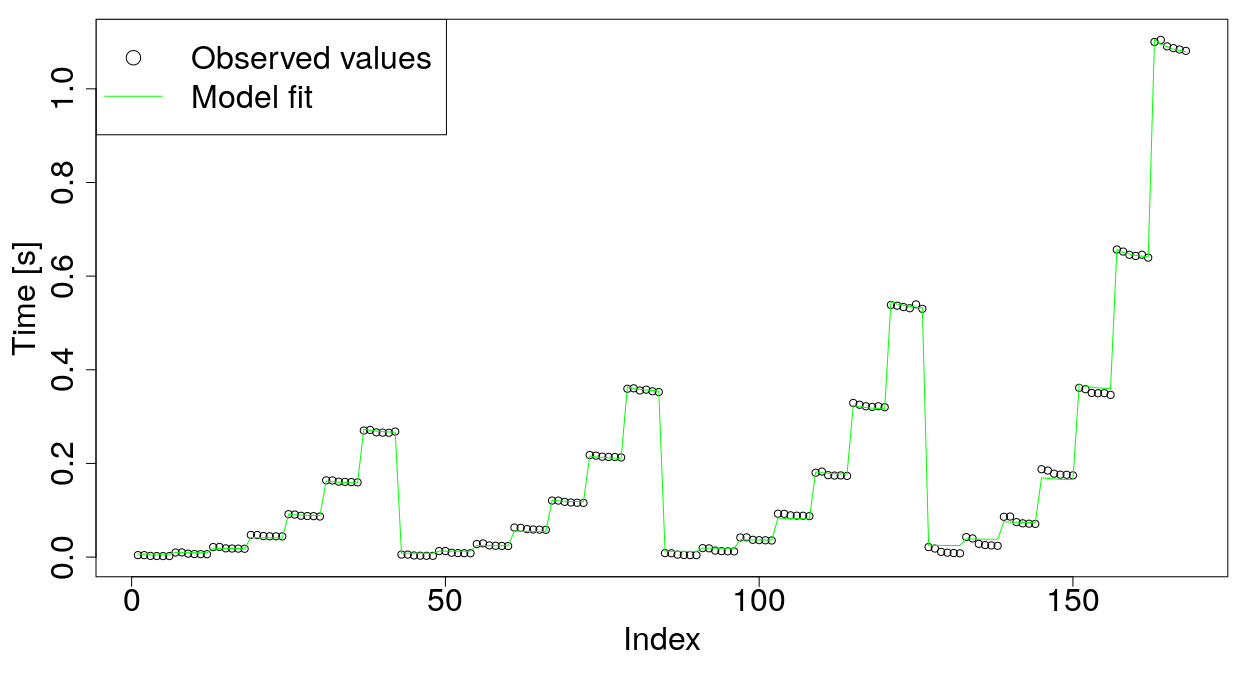
\includegraphics[scale=0.22]{figures/actionK-HTFETI.png}
%\end{minipage}
%\hfill
%\begin{minipage}{0.3\linewidth}
%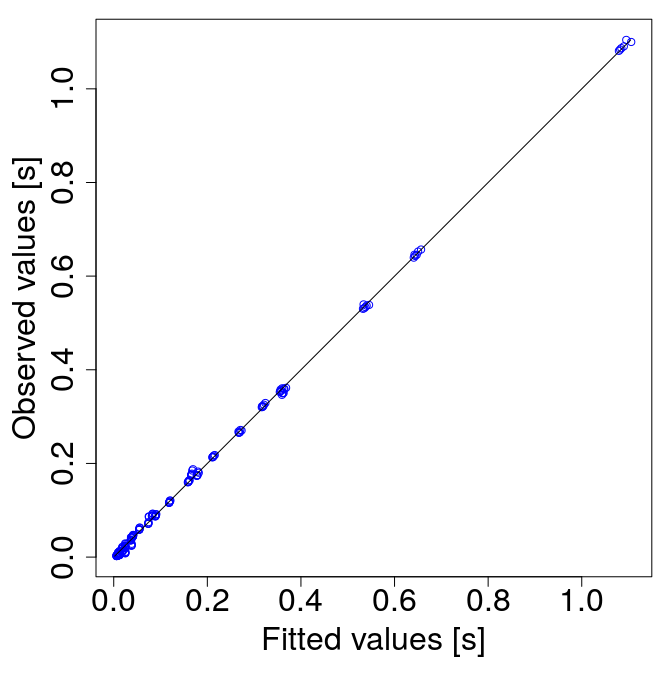
\includegraphics[scale=0.22]{figures/actionK-HTFETI-FvO.png}
%\end{minipage}
%}
\caption{Action of $K$ in HTFETI}
\label{fig:actionK-HTFETI}
\end{figure}

\paragraph{The remaining partial models} describe:  %listed in the Appendix \ref{sec:partialModels}. Those models describe 
assembling ($t_{K|asm}$), factorization ($t_{K|fact}$) and action ($t_{K|act|T}$,$t_{K|act|HT}$) of the stiffness matrices $K_i$ for all subdomains; assembling ($t_{Dir|asm}$) and action ($t_{Dir|act}$) of Dirichlet preconditioner for all subdomains; action of the Lumped preconditioner $t_{Lump|act}$ for all subdomains, assembling ($t_{GG^T|asm|T}$,$t_{GG^T|asm|HT}$) and action ($t_{GG^T|act|T}$, $t_{GG^T|act|HT}$) of the coarse problem $GG^T$, assembling the HTFETI objects ($t_{S\alpha|asm}$, $t_{F_0|asm}$). The $_{|T}$ stands for  Total FETI and $_{|HT}$ stands for HTFETI. 